\begin{document}

\chapter{Introduction}
\section{An introduction to Global navigation satellite systems}
The human presence in space began with the launch of the Soviet Union's Sputnik, closely followed by the USA's Explorer satellites in 1957 and 1958 respectively. Since then, many more launches of human-made objects into space have been performed, by several different countries. For the purpose of positioning there exist several systems in parallel, among them the US "Global Positioning System" (GPS), the Russian "Globalnaja Navigatsionnaja Sputnikovaja Sistema"[Latin transliteration] (GLONASS) and the Chinese \begin{CJK}{UTF8}{gbsn}北斗
\end{CJK}(Eng: Beidou) are arguably the most well known. The general name for satellite systems used for navigation purposes is the "Global Navigation Satellite System" (GNSS).
\section{Satellite orbits}
Some satellites used for e.g. radio and television are in an orbit around the earth at the same angular velocity as the planet's rotation, known as a geostationary orbit which implies that the satellite will stay over the same point on the surface of the earth. These satellites will travel along an orbit with a radius of 42.000 km or at a distance of around 36.000 km above the Earth's surface \cite{soop1994handbook}. 
\par
The GNSS satellites travel at a shorter distance and thus have a shorter orbital period. For the GPS system, the average distance is 20.200 km which gives them a base orbit period of around $\frac{1}{2}$ day. The other GNSS systems behave similarly to this. The distance to Earth is not constant over time since the satellite orbits will in practice always have some level of eccentricity, meaning that their path is elliptic with a center that may be far from the Earth's center. For navigation satellites, this eccentricity is generally small, below 0.02 meaning that the orbit is close to a circle \cite{Jeffrey}.
\par
The skyplot of GPS-satellites, in relation to the receiver's position from real observations is shown in figure \ref{fig:skyplot}. The plots are shown for satellite positions over the horizon and degrees clockwise from the north direction. The method for calculating the satellite position will be presented in section \ref{chap:ephPositioning}.
\begin{figure}[h!]
\centering
\begin{subfigure}{0.8\textwidth}
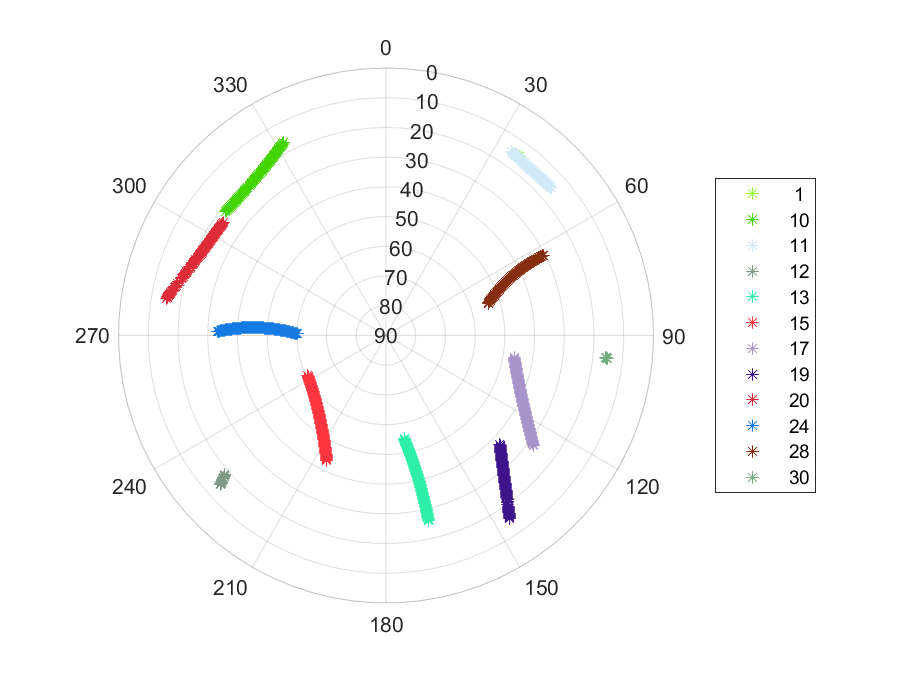
\includegraphics[width=\textwidth]{Introduction/elAz}
\subcaption{Elevation in degrees over the horizon on radial axis and degrees clockwise from north direction on the angular axis.}
\end{subfigure}
\begin{subfigure}{0.8\textwidth}
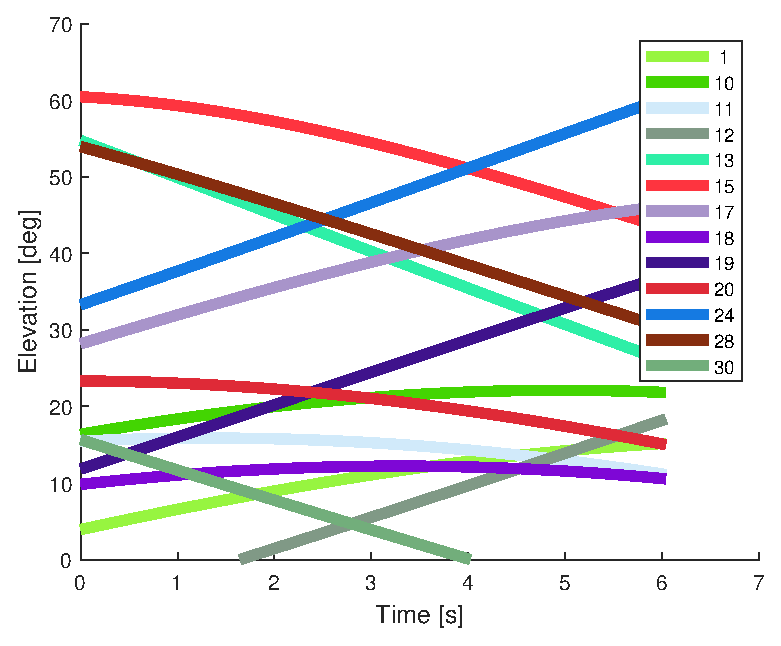
\includegraphics[width=\textwidth]{Introduction/elev}
\subcaption{Elevation in degrees over the horizon over time.}
\end{subfigure}
\caption{\label{fig:skyplot} Skyplot of GPS-satellites in the sky over the receiver, recorded on April 11$^{\text{th}}$ 2019, for one hour from 08:46 UTC. In (a), satellites are only plotted for when they are observed. Observations made in Stockholm, Sweden.}
\end{figure}



\section{The idea of satellite navigation}\label{IdeaSatNav}
The process of determining a GNSS-receiver's position on earth is based on comparing its distance to a number of satellites whose position is known by the receiver in a process called trilateration. The idea is illustrated in an ideal and noise free 2-dimensional case in figure \ref{fig:Trilateration} for two, three and four senders. The circles represent the radial distance to a satellite. For 2 senders, the solution is generally underdefined as multiple positions are valid. In a planar case that is illustrated with the two dots. In a 3D case, the solution space would form a circle at the intersections of the radius spheres. A unique solution only exists if both observations are equal to the corresponding radiuses and the circle collapses to a point. For three senders a unique solution is available and for four or more the system is overdetermined.
\begin{figure}[h!]
\begin{minipage}[t]{0.3\textwidth}
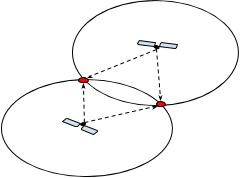
\includegraphics[width=\textwidth]{Background/BasisGNSS2Sat}
\end{minipage}
\begin{minipage}[t]{0.3\textwidth}
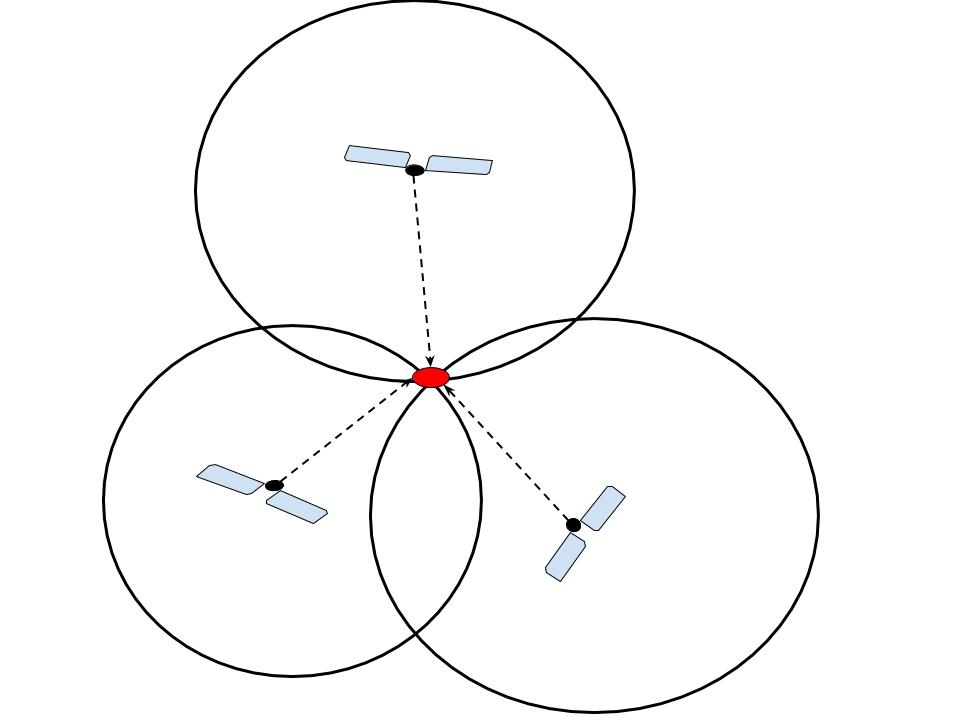
\includegraphics[width=\textwidth]{Background/BasisGNSS3Sat}
\end{minipage}
\begin{minipage}[t]{0.3\textwidth}
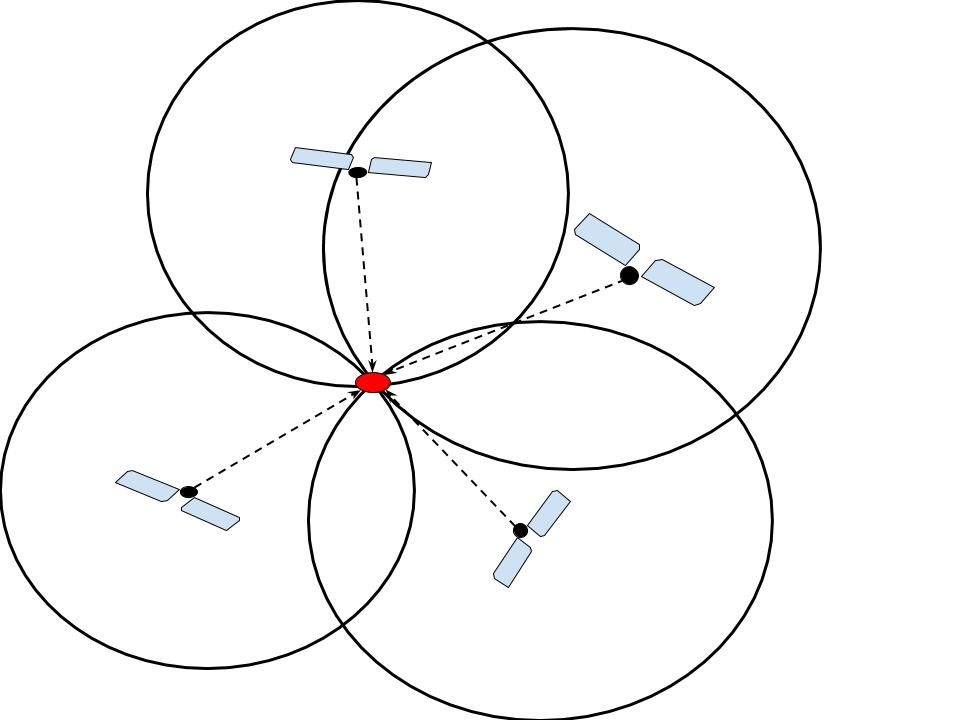
\includegraphics[width=\textwidth]{Background/BasisGNSS4Sat}
\end{minipage}
\caption{\label{fig:Trilateration} Example of positioning based on radial distance between sender and receiver for 2 (left), 3 (middle) and 4 (right) senders. The circles represent the distance from the sender and should be spherical, but is illustrated in 2D.}
\end{figure}

\section{Applications of GNSS-positioning}
The use of GNSS-positioning has spread from its original military purpose to being an integrated part of many applications, both business and consumer-oriented. The usage of positioning through satellite navigation is today widely spread and has numerous applications, such as being present in many modern cellphones, ships and cars. The advantages include its global usability for outdoor conditions as well as providing accuracy mostly within 5 meters at any time of the day \cite{posAccuracy}.
\par
In some applications, only the relative position between two units is of importance, e.g. for a ship docking or when landing on a platform. In this context the absolute position may be irrelevant and an offset from the true position does not influence the process, provided that both estimates contain the same offset. The simplest method of getting a relative position given two global positions is to calculate the difference between the positions. If a very high precision of the relative estimate is required, meaning that the error in the relative position estimate must be very low, this method may be insufficient as any error in the estimate of individual global positions may sum to a larger error. Then the use of some other technique which is better able to reduce the effect of the noise into the estimate may be superior to the trivial relative method. Different techniques have been developed to achieve a significantly higher precision than that available from standalone positioning. A few of these techniques  will be presented in section \ref{DGPSRTK}. 
\par
In the future, the use of satellite positioning may become an even more integrated part of our society as the potential to obtain a position estimate correct to within a few centimetres may lead to revolutions in many industries. Two examples are farming, when tractors may work the field unsupervised virtually without overlap in its path \cite{garcianoglobal} or the potential for autonomous delivery of medical or customer goods using drones \cite{Patrik2019}. 


\section{Other satellite navigation techniques}\label{DGPSRTK}
Three techniques which build on the idea presented in section \ref{IdeaSatNav} worth describing briefly are the differential technique, Differential GPS (DGPS) and Real Time Kinematic (RTK). 
\par
Differential techniques are based on using the direction to a transmitter rather than its position to estimate a relative distance between two points. The methods use that the scalar product between the direction vector and the relative distance is equal to the difference in distance to the transmitter. This way a relative position between two receivers can be calculated. Differential methods can be implemented as single, double or triple difference, where the use of double difference (DD) will be important in this paper. 
\par 
DGPS is a form of differential technique where a base station with a known position is used for reference. The base station can then transmit correction factors for the satellite signals to the other receiver, called a rover.
\par
The RTK method is a further development of the differential techniques, which utilizes the difference in phase between the signal for a base station and the mobile receiver. Commonly the L1 and L2 band of respectively 1575.42 MHz and 1227.60 MHz are used, which results in a wavelength of around 20 cm. The number of cycles between the receivers needs to be calculated. If the number of cycles is correct, the position can be calculated at a very high accuracy from the difference in phase. 

\section{Previous research}\label{previousResearch}
GNSS systems have been available for decades and much research has been performed on the behavior of the systems. Specifically, on the topic of the DD technique, research presented in \cite{BLUE} shows an implementation of a weighted least squares solution based on the signal strength for a pair of stationary receivers on a rooftop. The error of the estimate is presented in relation to the true baseline, where for two different baselines of 3 m and 8 m respectively, an error of respectively 3.2 m and 3.6 m is presented. 
\par 
In \cite{posAccuracyEnvironment}, research on similar techniques as in \cite{BLUE} is presented. One addition is that the estimates are performed in different environments with a 3 m baseline. For an open space environment, a mean error of 0.6-0.7 meter is achieved, for an environment with surrounding trees the measures mean error was 4 m and in the vicinity of buildings 2.3 m which indicate that noise levels in the observations may be very dependant on the environment. As stated in the article: "This indicates that obstacles such as buildings and trees cause higher noise of GPS measurements".
\par
In \cite{farrell1999global}, the DD-technique is presented which achieves an error in position fix of less than 1 m error for the receiver positions is. This is an example based on an experimental setup where any noise stemming from signal reflection can be expected to be zero as the receivers share the antenna between them and is unlikely to be achieved for real applications.
\par
In \cite{monteiro2005accuracy}, the performance of DGPS is evaluated as a function of the distance to the base station. The results from measurements from stationary DGPS receivers at a known distance show that the position with 95\% probability is correct to within 0.5-1 m near the base station and grows with 0.2 m per 100 km separation. 
\par
In \cite{feng2008gps} an RTK-solution is implemented and tested for baselines of 2-31 km, showing an accuracy of respectively 1 cm and 2 cm horizontally and vertically.
\end{document}
 
\section{Problem description and results}
This report presents the work that has been done with computing a relative position for the GNSS-INS receiver provided by inertial sense. It is a multi-sensor unit where either measurements from a single sensor, or the fused information from several, can be extracted. The data from "MEMs gyros, accelerometers, magnetometers, barometric pressure, and GPS/GNSS is fused to provide optimal estimation"\footnote{\url{https://inertialsense.com/\%C2\%B5ins-dual/} (2019-12-11)}. Data has been logged by sampling from stationary sensors and processed using MATLAB. 
\par
The results are based on the raw GNSS observation data sampled from the units and are presented in two ways: The relative position from the units from
\begin{enumerate}[(i)]
\item A difference between individual position estimates. \label{method(i)}
\item A Double Difference method. \label{method(iii)}
\end{enumerate}
The results show that for (\ref{method(i)}), the mean error can be expected to be in the magnitude of slightly above 5 m, with measurement mean values of 5 and 5.6 m. For (\ref{method(iii)}) the position error can be expected to be slightly below 5 m, with measurement mean values of 4.9 and 4.8 m. For future work a few improvements are suggested: data from other sensors may be fused to produce an even finer solution as well as the solution being produced in real-time. In addition to that, implementing a filter should be able to reduce much of the high frequency noise in the observations and lower the mean error.
\section{Objective} \label{sectionObjective}
The objective of this report is to investigate the relative positioning estimate based on two different methods and compare them. The two algorithms which are implemented are based on difference between the positions in the individual position estimates and the DD-based relative position. The results are presented for standard deviation in position per direction and the calculated mean error.
\section{Scientific question}
The purpose of this paper is to investigate what precision in the positioning that can be expected from a GNSS-solution for the purpose of the automated landing process. This is reflected in the question, formulated below.
\begin{itemize}
\item What precision can be expected from a relative GNSS-solution between two receivers using difference in global position fix and differentiated methods.
\end{itemize}
Ideally an estimate that is correct to within half a meter would ensure that the landing can be made safely.

\section{Delimitation}
Many applications, such as those mentioned above, are implemented as solutions to mobile problems. This investigation is limited to sampling from two receivers under stationary conditions, using a known distance. The results are also only presented for solutions presented from logged data. No real-time solution is implemented.

